%!TEX output_directory = <<temp>>
%!TEX copy_output_on_build = true

\documentclass[11pt]{article}

\usepackage[utf8]{inputenc}

\usepackage{amsmath}		% lets you input equations in math mode
\usepackage{graphicx}		% lets you include images
\usepackage{enumerate}		% lets you make lists
\usepackage{hyperref}		% lets you make links
\usepackage{subcaption}     % if you want to use subcaptions
\usepackage[all]{hypcap}	% makes links refer to figures and not captions
\usepackage{relsize}		% lets you use relative font sizes
\usepackage{caption}        % lets you add captions
\usepackage{array}          % lets you specify table column widths
\usepackage{float}
\usepackage{array}
\usepackage{cellspace}
\usepackage[margin=1in, paperwidth=8.5in, paperheight=11in]{geometry} %
\usepackage{xcolor}
\usepackage{natbib}
\usepackage{bibtopic}

\setlength\cellspacebottomlimit{8pt}
\newcommand\cincludegraphics[2][]{\raisebox{-.3\height}{\includegraphics[#1]{#2}}}

% place graphics in ./img/
\graphicspath{ {img/} }

\begin{document}



\title{Numerical Solver for Airflow}
\author{Bogdan Vitoc \\ William Fairman \\ Chris Lather}
% \date{date here} % leave this commented to display the current date
\maketitle



\begin{abstract}
   In this project, we apply concepts from vector calculus to find the airflow around any 2-dimensional shape. We make the assumptions that air is an incompressible and irrotational fluid in order to reduce the scope of our project while maintaining a realistic outcome for subsonic air speeds. We use the relaxation algorithm to solve Laplace's equation and ghost points to enforce a Neumann boundary condition at our surface boundary. We succeeded in producing vector-plots and animations visualizing the air velocity around an object.
\end{abstract}


\section{The Velocity Field}
Our velocity field ($\vec{V}$) consists of a fluid and an impermeable region for the fluid to flow around. In order to compute ($\vec{V}$), we have to implement a set of governing equations that produce favorable characteristics. In our case, we decided to make the velocity field irrotational and incompressible by implementing the following equations.

\begin{align}
    \nabla \times \vec{V} = 0 \label{nocurl} \\
    \nabla \cdot \vec{V} = 0 \label{nodiv}
\end{align}

By setting the curl of $\vec{V}$ to 0 (Eq. \ref{nocurl}), $\vec{V}$ is now considered path-independent and can be referred to as the gradient of a potential field. This potential field is known as the velocity potential field and is referred to as $\Phi$. If the divergence of $\vec{V}$ is also equal to 0 (Eq. \ref{nodiv}), then we can claim that $\Phi$ is a minimal surface defined by Laplace's equation 

\begin{align}
    \nabla^2 \Phi = 0
\end{align}

In this case our velocity potential is now a scalar field that represents the minimal amount of energy across the system: allowing the gradient of such a field to accurately represent fluid flow. 

%%This section needs more explanation
%%Include paragraph about why this is true. Characteristics fo minial surface, %%trade-off of our assumptions

\section{Relaxation Method}
The numerical solution to solve the Laplacian of a scalar field can be found through various algorithms. One of the most simple ways to solve the Laplacian is to set each point in the field equal to an average of it's neighbors. This method, known as relaxation, is an iterative approach to finding the Laplacian and fully solves the equation at $\text{time} = \infty$. For our velocity potential field, the value for each discrete fluid point is equal to

\begin{align}
 \Phi_{i,j} = \frac{\Phi_{i-1,j} + \Phi_{i,j-1} + \Phi_{i,j+1} +\Phi_{i+1,j} }{4}
\end{align}


\section{Surface Condition}
The above equations are able to satisfy the conditions for airflow outside the boundary of our object. However, we must add one more parameter to our solution to account for the airflow at the surface of our boundary. For these models, air does not flow through the object. In order to prevent airflow through an object, we must define the $\vec{V}$ to be tangent to the surface of the object. This is true when the dot product between the velocity vector and normal vector of the surface is equal to 0.

\begin{figure} [H] % H: forces layout according to position in the source
	\centering
	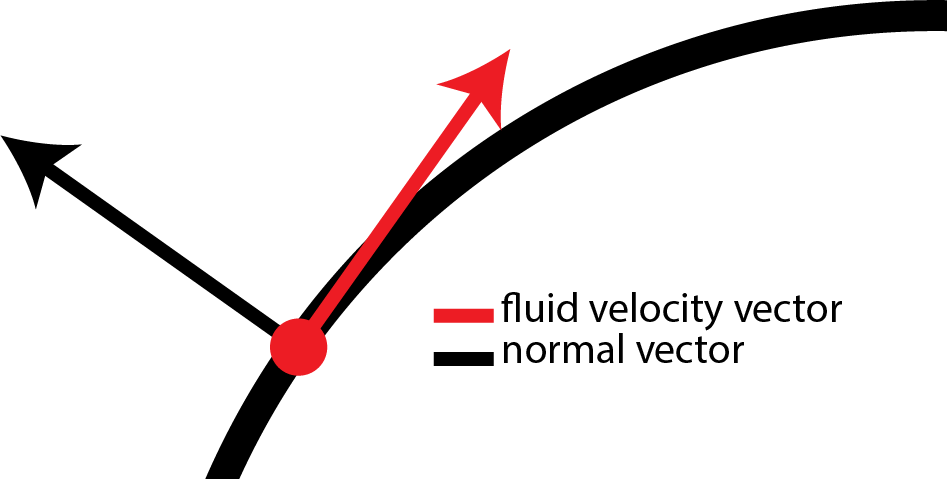
\includegraphics[width=0.5\textwidth]{lin_surface_condition.png}
	\captionsetup{margin={0.2\textwidth,0.2\textwidth}}
	\caption{Our simulation is considered realistic when the fluid velocity at the surface is anti-parallel to the normal vector at the surface.}
	%\caption*{\small (Egestas Justo Commodo)}
	\label{components}
\end{figure}

$\vec{V}$ can be re-written as the gradient of $\Phi$ and the equation can be reduced to

\begin{align}
    \text{grad}(\Phi) \cdot \hat{\textbf{n}} = 0
\end{align}

In order to make this condition true, we must set discrete points within the surface to a value that will eventually remove any perpendicular components of airflow when the relaxation method is applied to the surface points. The internal points that are manipulated to satisfy the surface condition are called ghost points.

\begin{figure} [H] % H: forces layout according to position in the source
	\centering
	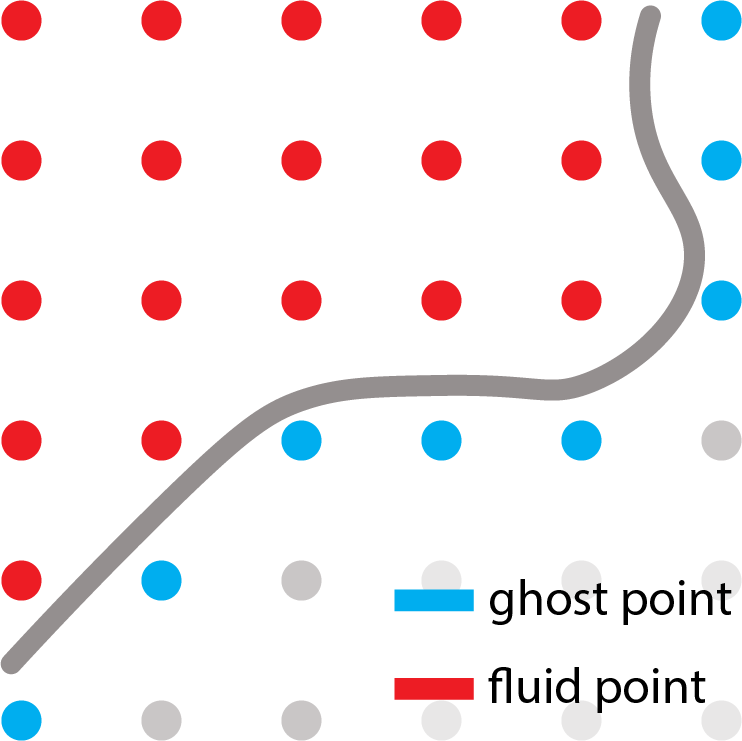
\includegraphics[width=0.4\textwidth]{lin_ghost.png}
	\captionsetup{margin={0.2\textwidth,0.2\textwidth}}
	\caption{A visualization of ghost points and fluid points bordering a surface. The continuous surface does not need to pass through a point in the numerical grid. Any point located directly on the surface would be classified as a fluid point.}
	%\caption*{\small (Egestas Justo Commodo)}
\end{figure}

\section{Ghost Points}
In order for a ghost point to affect a fluid point, the ghost point must touch the fluid point along one of its cardinal sides (North, South, East, West). Flipping this logic around gives us the conditions for selecting our ghost points. If a point internal to the surface comes into contact with a fluid point along one of its cardinal sides, that internal point is a ghost point because it has the ability to make the boundary condition true.

\subsection{Setting Values}
To find the appropriate value for a ghost point, we must take a closer look at the boundary condition for $\vec{V}$.

\begin{align}
    \text{grad}(\Phi) \cdot \hat{\textbf{n}} = 0 \\
    \begin{bmatrix} \frac{\partial\Phi}{\partial x} \\[6pt] \frac{\partial\Phi}{\partial y} \end{bmatrix}
    \cdot
    \begin{bmatrix} X_n \\  Y_n \end{bmatrix} = 0
\end{align}

If we choose our surface to be a straight horizontal line, the normal vector can be reduced to:
\begin{align}
    \begin{bmatrix} X_n \\  Y_n \end{bmatrix}
    =
    \begin{bmatrix} 0 \\  1 \end{bmatrix} 
\end{align}

This allows us to further refine our boundary condition:
\begin{align}
    \text{grad}(\Phi) \cdot \hat{\textbf{n}} = 0 \\
    \begin{bmatrix} \frac{\partial\Phi}{\partial x} \\[6pt] \frac{\partial\Phi}{\partial y} \end{bmatrix}
    \cdot
    \begin{bmatrix} 0 \\  1 \end{bmatrix}  = 0 \\ 
    \frac{\partial\Phi}{\partial y} = 0
\end{align}

When we implement a discrete representation of $\frac{d\Phi}{dy}$,we can now claim that:
\begin{align}
    \frac{\partial\Phi}{\partial y} &= \frac{\Phi_{i,j+1} - \Phi_{i,j-1}}{2} = 0 \\
    \Phi_{i,j-1} &= \Phi_{i,j+1}
\end{align}
The value of each ghost point is selected by copying the value of a point mirrored directly across the surface, called the mirror point. If we make the ghost point equal to its mirrored fluid point, the normal component of the gradient between the two values of $\Phi$ will be 0, satisfying the boundary condition. Conceptually, by setting an inner ring of ghost points equal to an outer ring of fluid points, we can guarantee the slope across the surface to be tangential (Fig. \ref{components}).

\begin{figure} [H] % H: forces layout according to position in the source
	\centering

	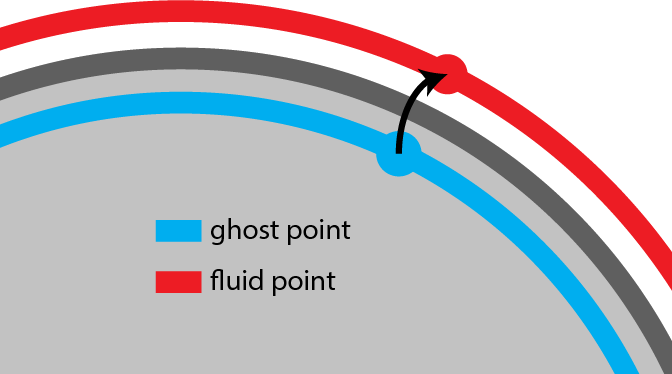
\includegraphics[width=0.6\textwidth]{lin_graphic.png}
	\captionsetup{margin={0.2\textwidth,0.2\textwidth}}
	\caption{Setting the ghost point equal to the value of its mirrored fluid point will satisfy the boundary condition.}
	%\caption*{\small (Egestas Justo Commodo)}
\end{figure}

%%Add image
However, in a discrete setting, the number of ghost points will always be less than the number of exterior fluid points because the perimeter of the fluid points coming into contact with the surface is larger than the perimeter of ghost points (at least on a surface without concavities).

\begin{figure} [H] % H: forces layout according to position in the source
	\centering

	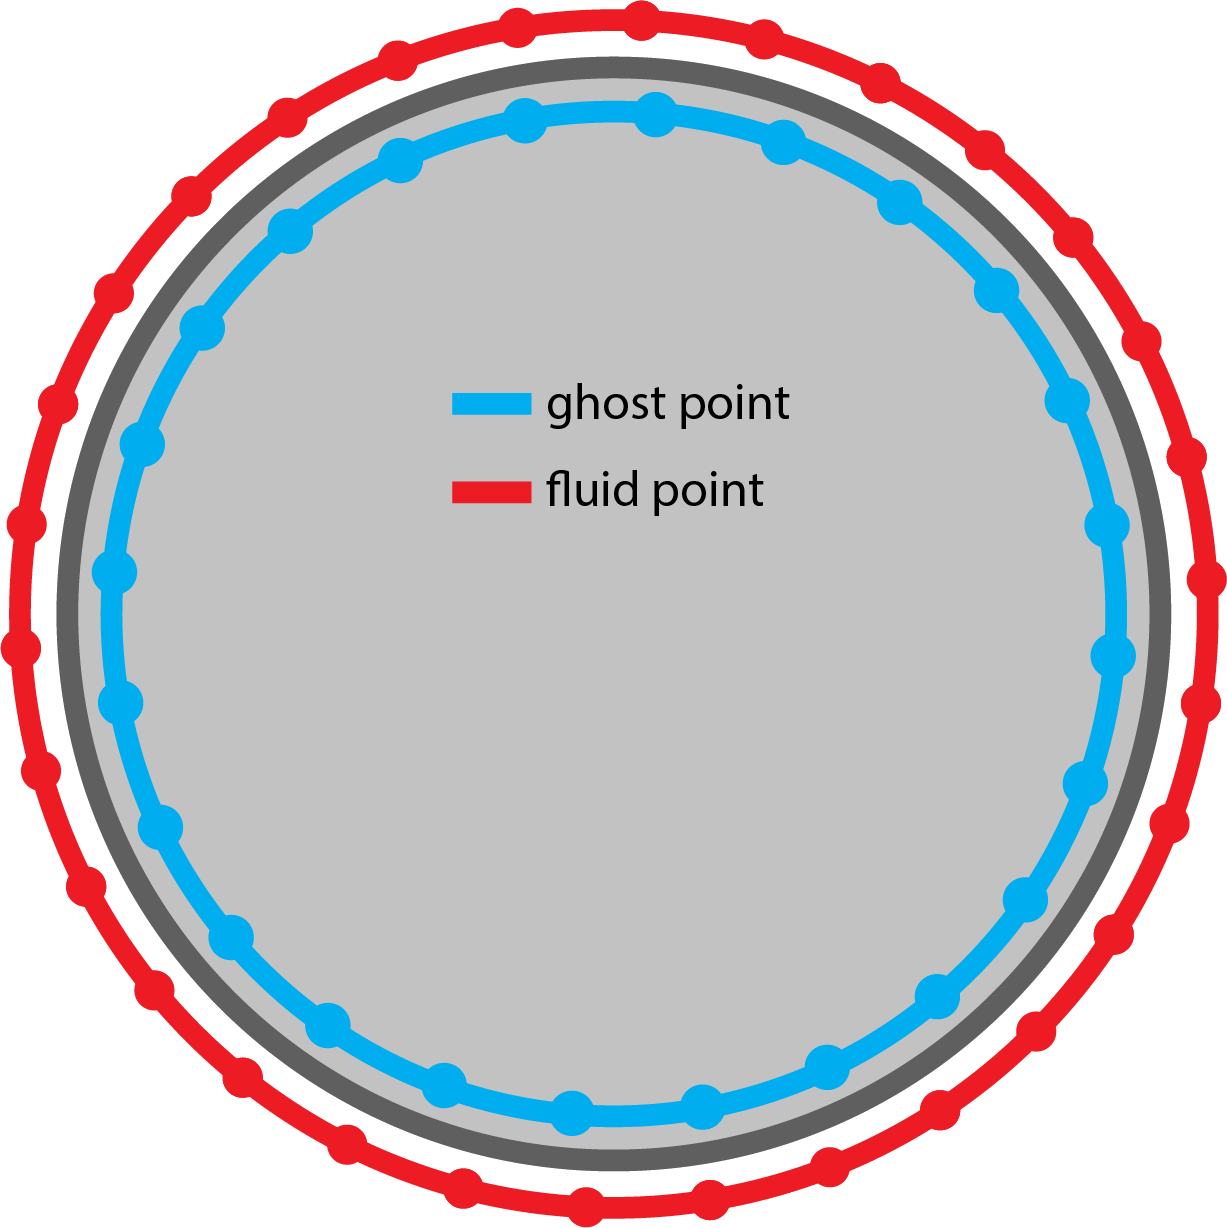
\includegraphics[width=0.40\textwidth]{lin_graphic_2.png}
	\captionsetup{margin={0.2\textwidth,0.2\textwidth}}
	\caption{The perimeter of fluid and ghost points is represented by two rings with discrete points equally spaced along both rings. The number of fluid points is larger than the number of ghost points}
	%\caption*{\small (Egestas Justo Commodo)}
\end{figure}

This inequality makes it difficult to find a fluid point that is a direct mirror of each ghost point. However, if we make the ghost points equal to a \textit{set} of fluid points nearby, we can force that area to be approximately equipotential.

\subsection{Stencil Average}
To approximate the value of our ghost points, we decided to equate each ghost point to the average value of all the fluid points it touches in a 25-point stencil. Other mirroring techniques are discussed in \cite{lekven2017verification}

\begin{figure} [H] % H: forces layout according to position in the source
	\centering

	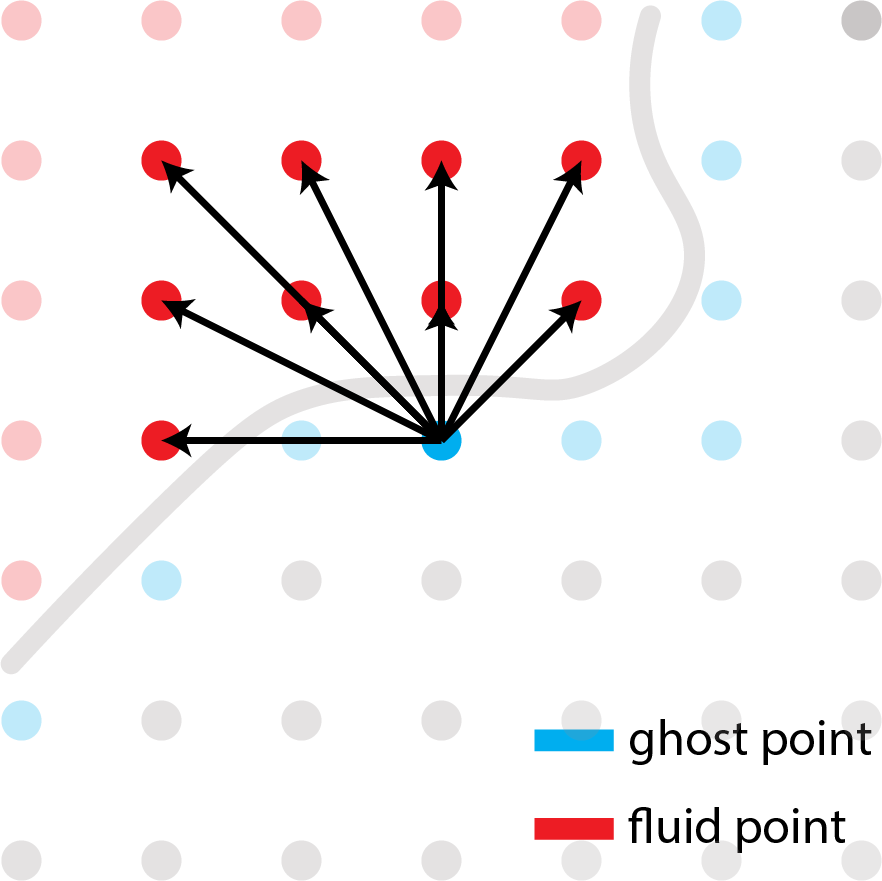
\includegraphics[width=0.4\textwidth]{lin_ghost_stencil.png}
	\captionsetup{margin={0.2\textwidth,0.2\textwidth}}
	\caption{Each ghost point mirrored from an average of its surrounding fluid points. One might accurately assume a 9-point stencil to be more reasonable. The 25-point average is an artifact of a flawed POV.}
	%\caption*{\small (Egestas Justo Commodo)}
\end{figure}

\subsection{Initial Conditions}
We need an exterior airflow to give our surface something to disrupt. We create this fluid flow by enforcing Dirichlet boundary conditions on all sides of our field. Since we want the air to be flowing to the right, the left side holds a positive velocity potential while the right side is held at 0. The top and bottom must be held at some value since the relaxation method does not work at a boundary. We choose to hold the top and bottom at zero as well.

\begin{figure} [H] % H: forces layout according to position in the source
	\centering
	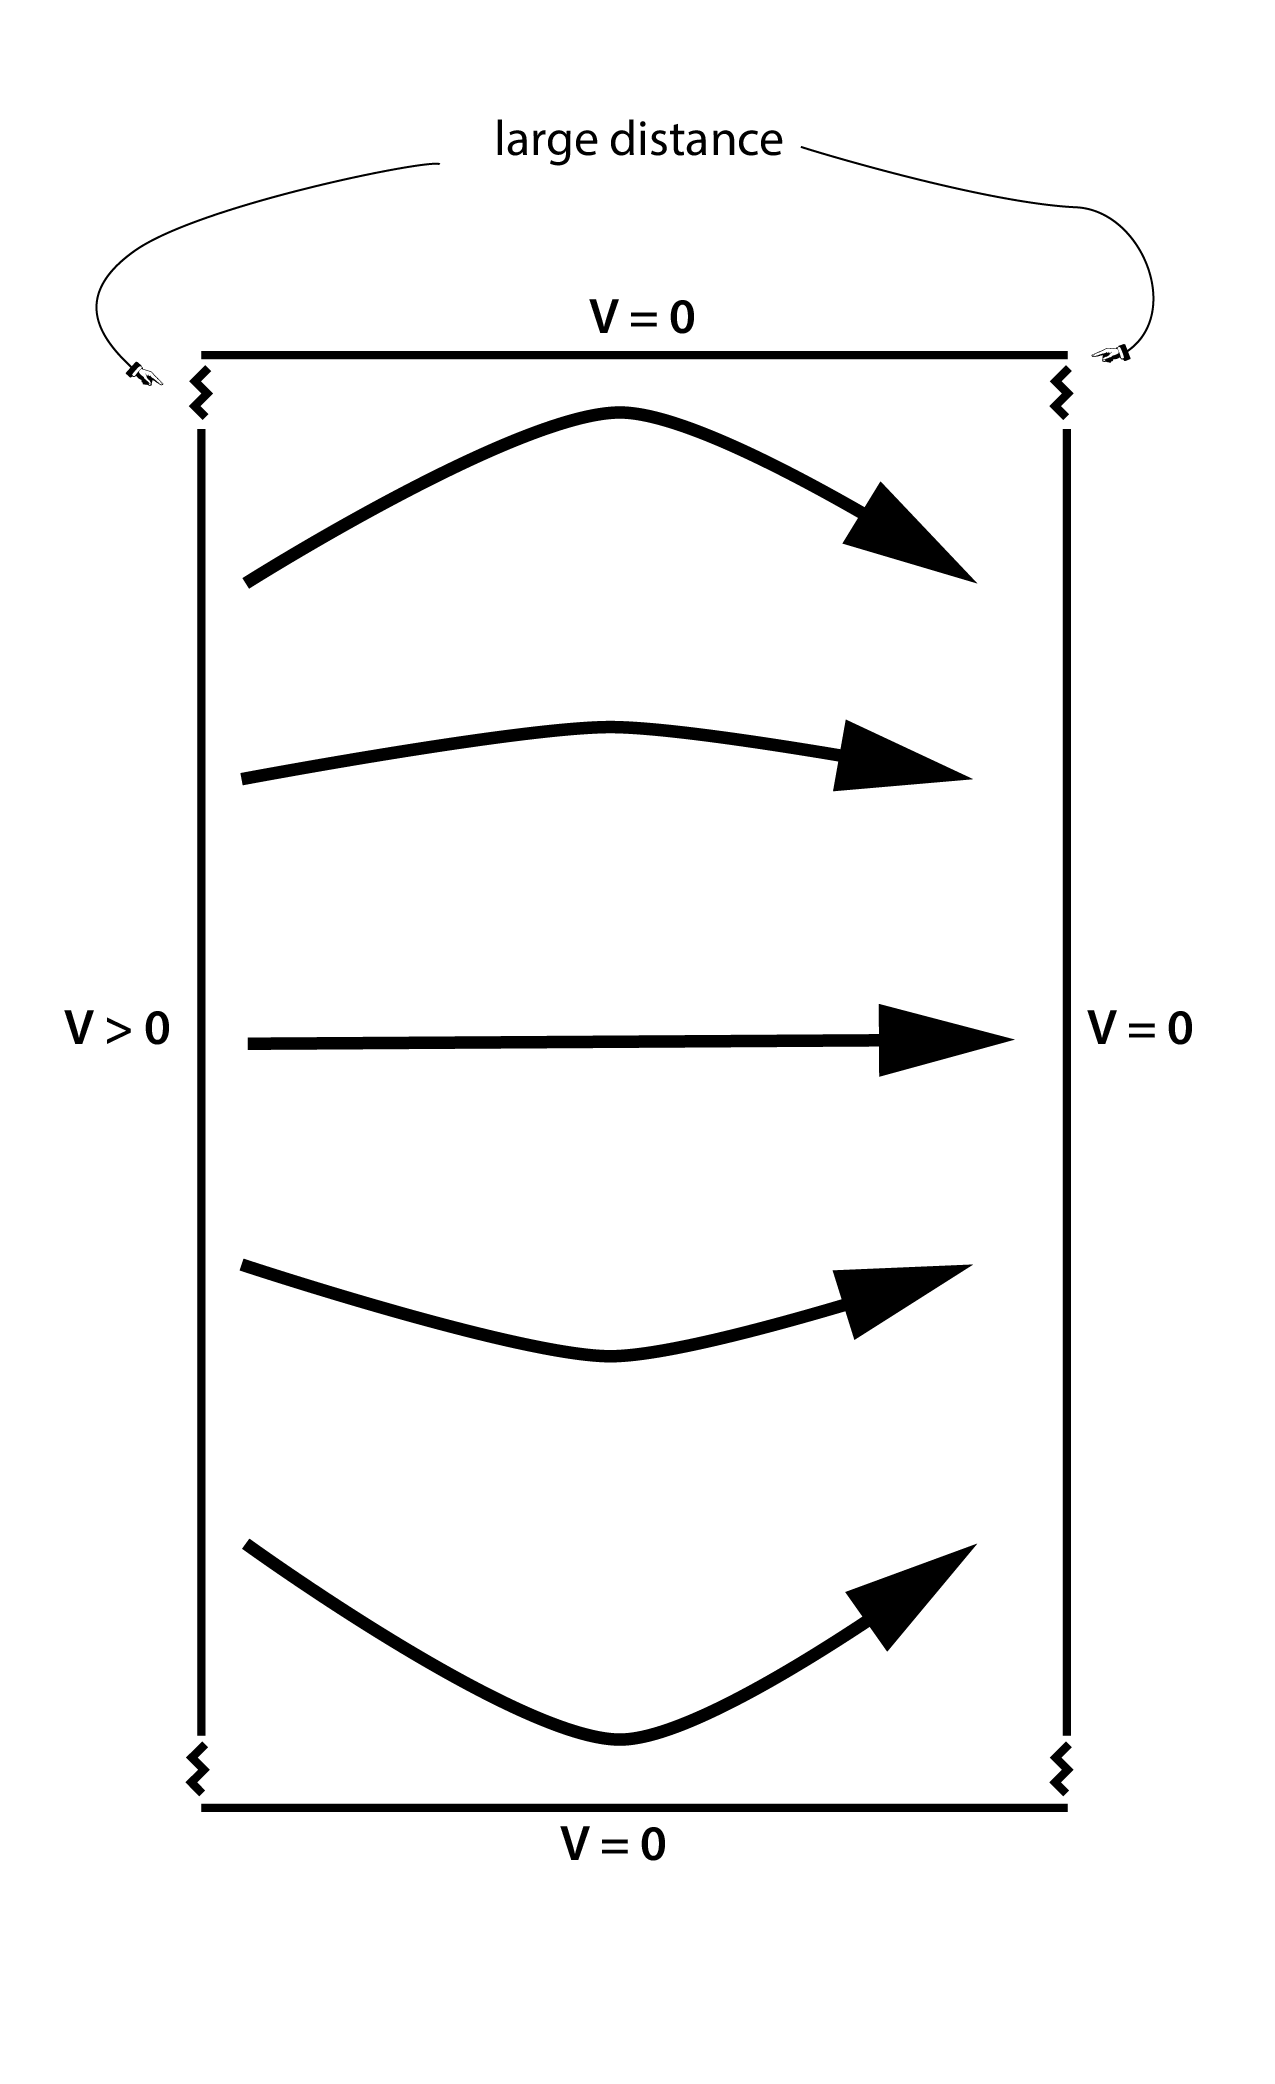
\includegraphics[width=0.4\textwidth]{initial_flow.png}
	\captionsetup{margin={0.2\textwidth,0.2\textwidth}}
	\caption{Initial air flow (e.g. from wind).}
	%\caption*{\small (Egestas Justo Commodo)}
\end{figure}

This does result in a non-parallel airflow most noticeably near the top and bottom. To counteract this effect we made our fluid domain very tall relative to our object. Alternatively the top and bottom sides could be given the same boundary condition as the shape, enforcing a parallel airflow, as if in a wind tunnel. Not only would this increase accuracy, but it would bring big savings in computation time.

\section{Results}
We decided to setup our simulation environment in Matlab over Mathematica due to its heightened abilities to handle numerical calculations. In order to take advantage of our numerical solver's ability to work for almost any surface, we needed an easy way to define and import complex surfaces. Our final program can convert black and white images into a discrete surface.

Our initial proof of concept was to model the airflow around an ellipse. The velocity potential field ($\Phi$) is shown below:

\begin{figure} [H] % H: forces layout according to position in the source
	\centering
	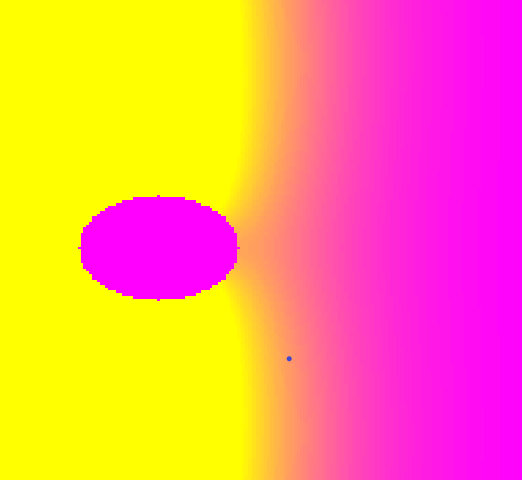
\includegraphics[width=0.5\textwidth]{flow.png}
	\captionsetup{margin={0.2\textwidth,0.2\textwidth}}
	\caption{Velocity potential around an ellipse.}
	%\caption*{\small (Egestas Justo Commodo)}
\end{figure}
In this example, $\Phi$ is represented as a color range between bright yellow and purple: where yellow is an area of high potential and purple is an area of low potential. The outline of our object can be seen as an area of low potential because the internal points of the object are set to 0.

The velocity vector $\vec{V}=\nabla\cdot\Phi$  can be shown when taking the gradient of the field.
\begin{figure} [H] % H: forces layout according to position in the source
	\centering
	
\includegraphics[width=0.5\textwidth]{flow_vec.png}
	\captionsetup{margin={0.2\textwidth,0.2\textwidth}}
	\caption{Vector field representing the gradient of the velocity potential field.}
\end{figure}
While the figure shows an accurate representation of airflow, the airflow as a whole is hard to visualize due to the size of the vector arrows. After modifying our code, we settled on representing airflow as a stream-line plot with $\Phi$ overlaid in the background.

\subsection{Airflow Graphics}
Below is a selection of figures that reflect the ability of our code to parse a black and white image and calculate the accompanying airflow. Each image has an accompanying video that can be found here: \href{https://drive.google.com/drive/folders/1YatS7map3rJvWgA_mO1nS_kQ8kbgIf8t}{https://drive.google.com/drive/folders/1YatS7map3rJvWgA\_mO1nS\_kQ8kbgIf8t}

\begin{figure} [H] % H: forces layout according to position in the source
	\centering
	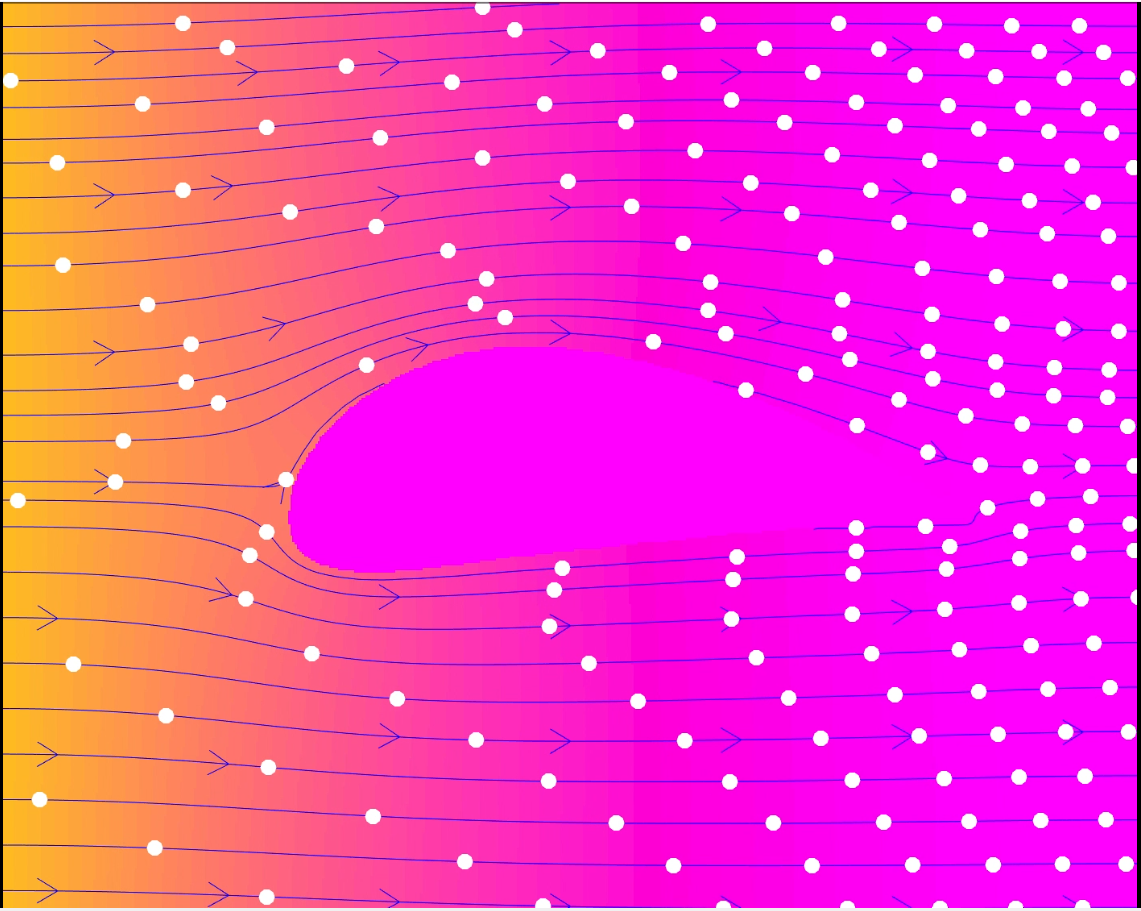
\includegraphics[width=0.6\textwidth]{airfoil.png}
	\captionsetup{margin={0.2\textwidth,0.2\textwidth}}
	\caption{Airflow around an airfoil.}
	%\caption*{\small (Egestas Justo Commodo)}
\end{figure}

\begin{figure} [H] % H: forces layout according to position in the source
	\centering
	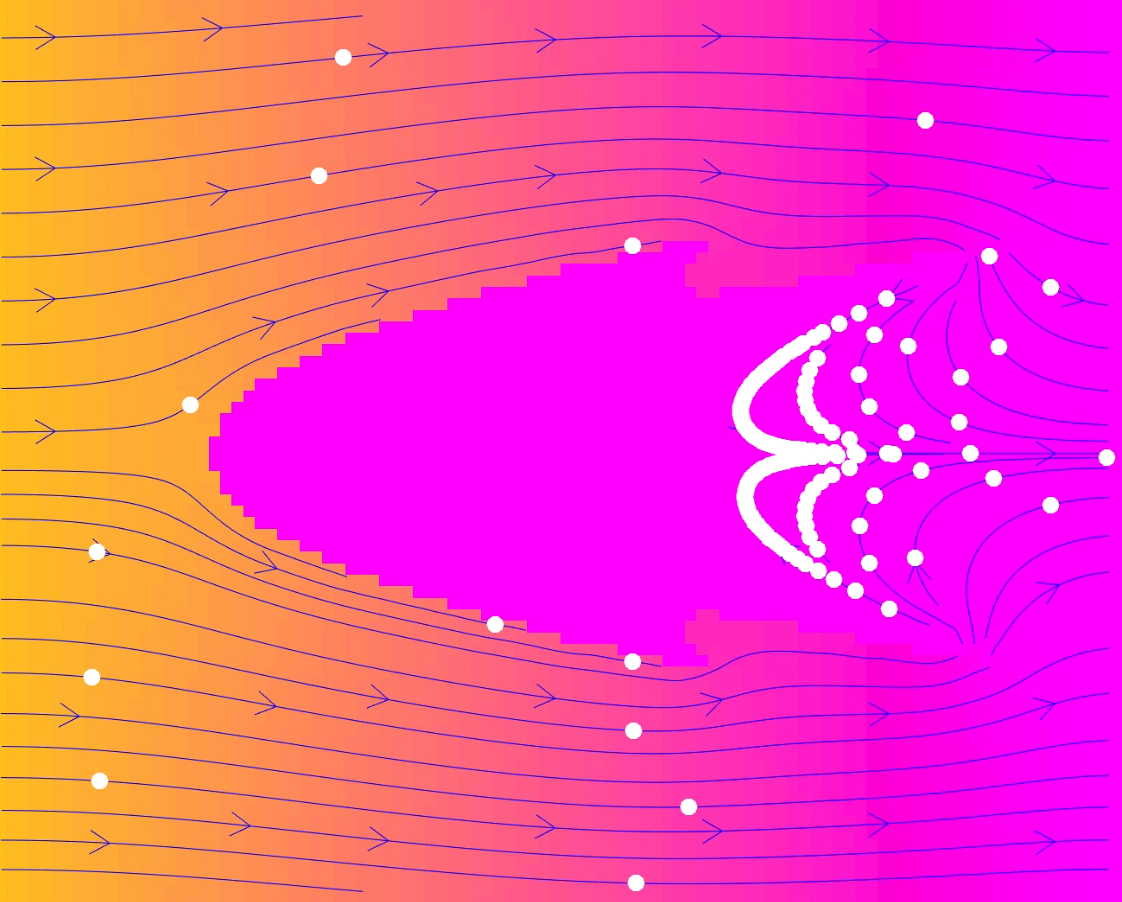
\includegraphics[width=0.6\textwidth]{arrowhead.png}
	\captionsetup{margin={0.2\textwidth,0.2\textwidth}}
	\caption{Airflow around an arrowhead.}
	%\caption*{\small (Egestas Justo Commodo)}
\end{figure}

\begin{figure} [H] % H: forces layout according to position in the source
	\centering
	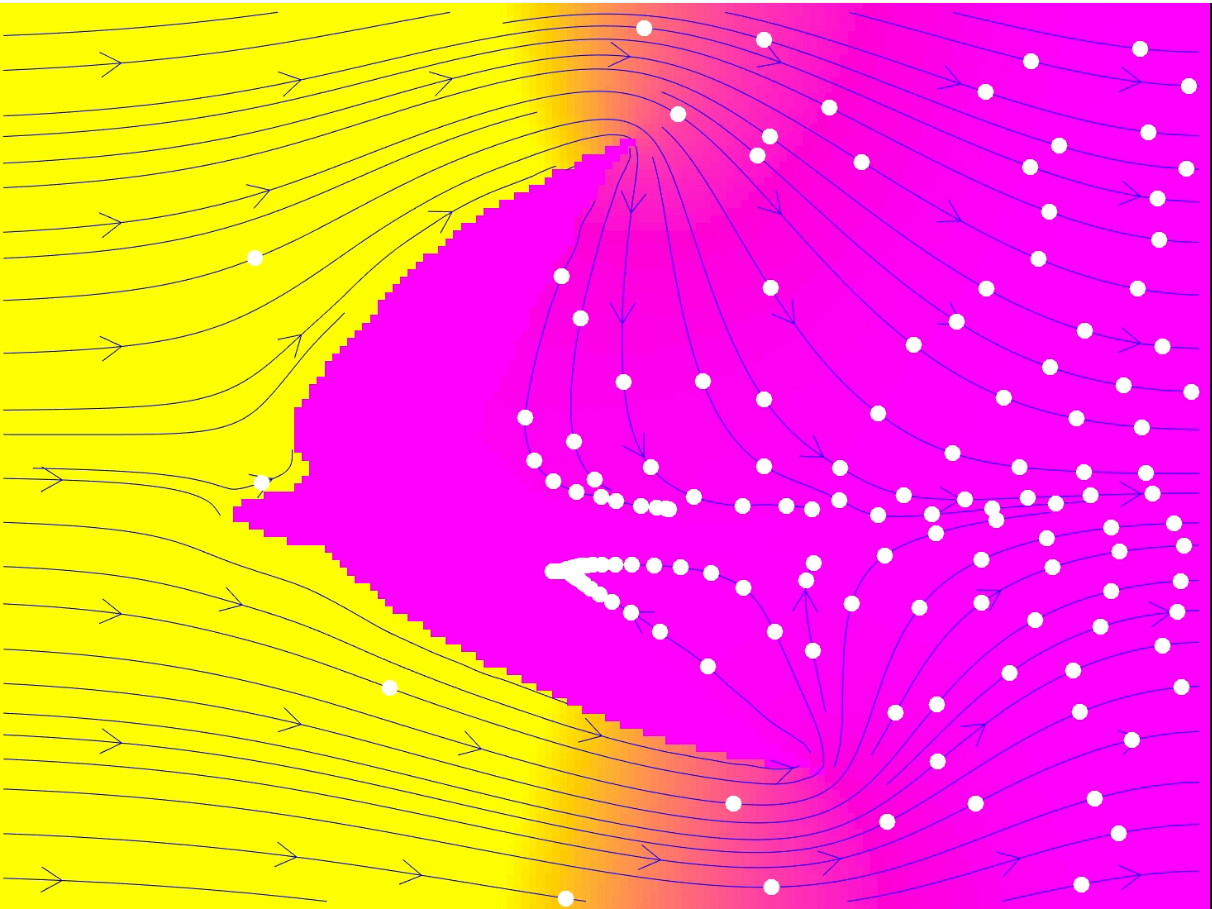
\includegraphics[width=0.6\textwidth]{swallow.png}
	\captionsetup{margin={0.2\textwidth,0.2\textwidth}}
	\caption{Airflow around an African Swallow carrying a coconut.}
	%\caption*{\small (Egestas Justo Commodo)}
\end{figure}

\begin{btSect}[abbrvnat]{references}
   \section*{References}
   \btPrintCited
\end{btSect}
 
\begin{btSect}[plainnat]{supplementary}
   \section*{Further Reading}
   \btPrintAll%  see manual for alternatives...
\end{btSect}

\end{document}

